\documentclass[12pt]{article}
\usepackage{../../ficha}

\begin{document}

\ficha{Proporcionalidade Inversa e Função Quadrática}[Proporcionalidade Inversa, Funções $y = ax^2$ e Interseção de Gráficos]

\instrucoes{Resolve os exercícios, apresentando os cálculos. Duas grandezas são inversamente proporcionais se o produto $x \times y$ é constante.}

\secao{Reconhecer Proporcionalidade Inversa}{Indica se as grandezas são inversamente proporcionais. Em caso afirmativo, indica a constante de proporcionalidade.}
\begin{exercicios}
  \item \begin{tabular}[c]{|c|c|c|c|c|}\hline
    $x$ & 1 & 2 & 4 & 8 \\\hline
    $y$ & 24 & 12 & 6 & 3 \\\hline
  \end{tabular}
  \item \begin{tabular}[c]{|c|c|c|c|c|}\hline
    $x$ & 2 & 3 & 5 & 6 \\\hline
    $y$ & 15 & 10 & 8 & 5 \\\hline
  \end{tabular}
  \item O número de operários e o tempo para fazer uma obra (todos ao mesmo ritmo).
  \item A velocidade de um carro e o tempo para percorrer 120\,km.
  \item O número de pessoas e o dinheiro gasto em bilhetes de cinema.
  \item O comprimento e a largura de retângulos com 36\,cm$^2$ de área.
\end{exercicios}

\secao{Problemas de Proporcionalidade Inversa}{Resolve.}
\begin{exercicios}
  \item 4 pintores pintam uma casa em 6 dias. Quantos dias levariam 3 pintores?
  \item Um carro a 90\,km/h faz uma viagem em 4 horas. Quanto tempo demora a 120\,km/h?
  \item Uma torneira enche um tanque em 10 horas. Quanto tempo demoram 5 torneiras iguais?
  \item Uma caixa de bombons dá para 12 crianças receberem 5 bombons cada. Se forem 15 crianças, quantos bombons recebe cada uma?
  \item Uma quantia foi dividida igualmente por 8 pessoas, cabendo 45 euros a cada uma. Quanto receberia cada pessoa se fossem 6?
  \item Sabendo que $x$ e $y$ são inversamente proporcionais e que $y = 8$ quando $x = 3$, escreve $y$ em função de $x$ e calcula $y$ para $x = 6$.
\end{exercicios}

\secao{Gráficos de Proporcionalidade Inversa}{Considera a função $f(x) = \dfrac{12}{x}$, com $x > 0$.}
\begin{exercicios}
  \item Completa a tabela: \begin{tabular}[c]{|c|c|c|c|c|c|c|}\hline
    $x$ & 1 & 2 & 3 & 4 & 6 & 12 \\\hline
    $f(x)$ & & & & & & \\\hline
  \end{tabular}
  \item Representa graficamente a função.
  \item O gráfico é uma reta? Como se chama esta curva?
  \item Determina $x$ tal que $f(x) = 1{,}5$.
  \item O ponto $(8;\ 1{,}5)$ pertence ao gráfico de $f$? Justifica.
\end{exercicios}

\secao{Funções Quadráticas $y = ax^2$}{Resolve.}

\begin{center}
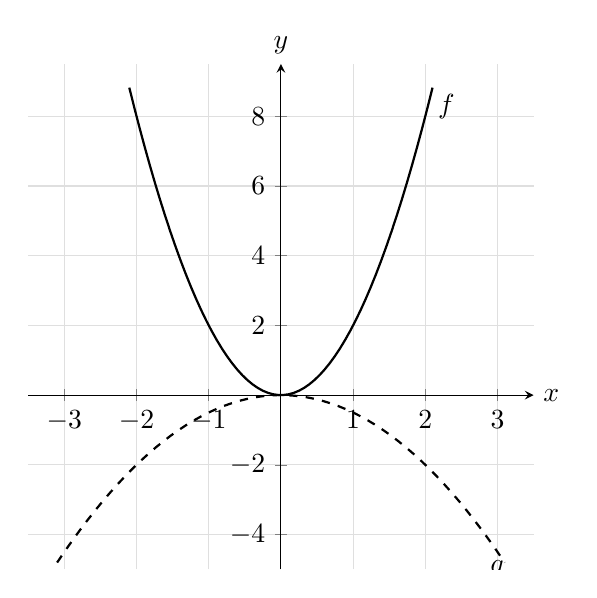
\begin{tikzpicture}
\begin{axis}[axis lines=middle, xmin=-3.5, xmax=3.5, ymin=-5, ymax=9.5, xtick={-3,...,3}, ytick={-4,-2,...,8}, grid=both, grid style={gray!25}, width=8cm, height=8cm, xlabel=$x$, ylabel=$y$, every axis x label/.style={at={(ticklabel* cs:1)},anchor=west}, every axis y label/.style={at={(ticklabel* cs:1)},anchor=south}]
  \addplot[thick, domain=-2.1:2.1, samples=60] {2*x^2} node[pos=0.97, right] {$f$};
  \addplot[thick, dashed, domain=-3.1:3.1, samples=60] {-0.5*x^2} node[pos=0.97, below] {$g$};
\end{axis}
\end{tikzpicture}
\end{center}

\begin{exercicios}
  \item Os gráficos de $f$ e $g$ são parábolas da forma $y = ax^2$. Usando pontos do gráfico, determina $a$ em cada caso.
  \item Indica o vértice e o eixo de simetria das duas parábolas.
  \item Qual das parábolas tem a concavidade voltada para cima? Como se relaciona isso com o sinal de $a$?
  \item Para $h(x) = 3x^2$, calcula $h(2)$, $h(-2)$ e $h(\tfrac{1}{3})$.
  \item O ponto $(4, 8)$ pertence ao gráfico de $y = ax^2$. Determina $a$.
  \item Ordena por abertura (da mais fechada para a mais aberta): $y = x^2$, $y = 4x^2$, $y = \tfrac{1}{4}x^2$.
  \item A área de um quadrado em função do lado é $A(\ell) = \ell^2$. Calcula $A(5)$ e determina $\ell$ quando $A = 49$.
\end{exercicios}

\secao{Interseção de Gráficos}{Determina, graficamente e analiticamente, os pontos de interseção.}
\begin{exercicios}
  \item $y = 2x + 1$ \; e \; $y = -x + 7$
  \item $y = x$ \; e \; $y = x^2$
  \item $y = 2x^2$ \; e \; $y = 8$
  \item $y = x^2$ \; e \; $y = 2x$
  \item $y = \dfrac{4}{x}$ \; e \; $y = x$, com $x > 0$
  \item Interpreta graficamente o sistema $\begin{cases} x + y = 5 \\ x - y = 1 \end{cases}$ e resolve-o.
\end{exercicios}

\secao{Desafios}{Resolve os problemas.}
\begin{exercicios}
  \item Uma obra é feita por 6 operários em 20 dias. Ao fim de 5 dias, juntam-se mais 3 operários. Quantos dias faltam para acabar a obra?
  \item A distância de travagem de um carro é $d = 0{,}006\,v^2$ (em metros, com $v$ em km/h). Qual é a distância de travagem a 50\,km/h? E a 100\,km/h? Duplicar a velocidade duplica a distância?
  \item Um retângulo tem área 48\,cm$^2$. Escreve o comprimento $c$ em função da largura $\ell$. Que tipo de função obtiveste?
  \item Determina $k$ de modo que a reta $y = k$ intersete a parábola $y = 3x^2$ nos pontos de abcissa $-2$ e $2$.
  \item Os gráficos de $y = ax^2$ e $y = 2x + 4$ intersetam-se no ponto de abcissa 2. Determina $a$ e o outro ponto de interseção.
\end{exercicios}

\end{document}
